\subsection{The Qutrit}
A system given by the Hamiltonian
\begin{equation}
\label{eq:Ham}
H = \sum_{j = 1}^2 \sum_{i =j}^{3} \omega_{ij}\ket{i}\bra{e_j}  + \frac{\Omega(t)_{a}}{2}\ket{a}\bra{e_2}  +\,\text{h.c}
\end{equation}
which is shown in Figure \ref{fig:Ham}.  It consists of two excited states, $\ket{e_1}, \ket{e_2}$, an auxiliary state $\ket{a}$ and the ground states $\ket{1}, \ket{2}, \ket{3}$ which 
makes up the computational basis of the qutrit. By a transformation of basis the Hamiltonian can be rewritten as 
\begin{equation}
\label{eq:Hamd}
H_d = \sum_{j = 1}^2 \frac{\Omega_j(t)}{2}e^{-i\phi_j}\ket{b_j}\bra{e_j}  + \frac{\Omega_a(t)}{2}\ket{a}\bra{e_2}  +\,\text{h.c}
\end{equation} 
by a Morris-Shore transformation\cite{morris}. Now one can find a dark state to this hamiltonian, an eigenstate with eigenvalue $0$, $H\ket{d} = 0$. In this basis for 3 fixed angles, $\theta, \varphi, $, there exists a normalized dark state $\ket{d} = \cos\theta\ket{1} + e^{i\chi}\sin\theta\cos\varphi\ket{2} + e^{i\xi}\sin\theta\sin\varphi\ket{3}$, additionally one can determine two states $\ket{b_1} = N_1 \left(-e^{i\xi}\sin\theta\sin\varphi\ket{1} + \cos\theta\ket{2} \right)$ and $\ket{b_2} = N_2 \left(\cos\theta\ket{1} +  e^{i\chi}\sin\theta\cos\varphi\ket{2} + \Lambda \ket{3}\right ) $, where $N_1, N_2$ are normalization factors and $\Lambda$ can be chosen such that $\bra{d}\ket{b_2} = 0$.

\begin{figure}[H]
\label{fig:Ham}
    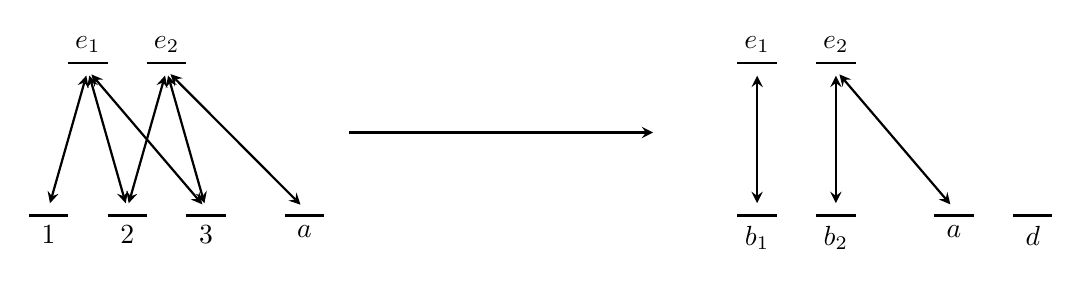
\begin{tikzpicture}[
      scale=0.5,
      level/.style={thick},
      virtual/.style={thick,densely dashed},
      trans/.style={thick,<->,shorten >=2pt,shorten <=2pt,>=stealth},
      arrow/.style={thick,->,shorten >=2pt,shorten <=2pt,>=stealth},
      classical/.style={thin,double,<->,shorten >=4pt,shorten <=4pt,>=stealth}]
      
    % Excited
    \draw[level] (5cm,0em) -- (6cm,0em) node[midway,above] {$\ket{e_1}$};    
    \draw[level] (7cm,0em) -- (8cm,0em) node[midway,above] {$\ket{e_2}$};
	% Ground states
    \draw[level] (4cm,-11em) -- (5cm,-11em) node[midway,below] {$\ket{1}$};
    \draw[level] (6cm,-11em) -- (7cm,-11em) node[midway,below] {$\ket{2}$};
    \draw[level] (8cm,-11em) -- (9cm,-11em) node[midway,below] {$\ket{3}$};
    \draw[level] (10.5cm,-11em) -- (11.5cm,-11em) node[midway,below] {$\ket{a}$};
    % e_1
    % Draw the transitions.
    \draw[trans] (5.5cm,-0.5em) -- (4.5cm,-10.5em) node[midway,left] {};
    \draw[trans] (5.5cm,-0.5em) -- (6.5cm,-10.5em) node[midway,left] {};
    \draw[trans] (5.5cm,-0.5em) -- (8.5cm,-10.5em) node[midway,left] {};
   	% e_2
    \draw[trans] (7.5cm,-0.5em) -- (6.5cm,-10.5em) node[midway,left] {};
    \draw[trans] (7.5cm,-0.5em) -- (8.5cm,-10.5em) node[midway,left] {};
    \draw[trans] (7.5cm,-0.5em) -- (11cm,-10.5em) node[midway,left] {};
    
    
    \draw[arrow] (12cm,-5em) -- (20cm,-5em) node[] {}; 
    
    % Excited
    \draw[level] (22cm,0em) -- (23cm,0em) node[midway,above] {$\ket{e_1}$};    
    \draw[level] (24cm,0em) -- (25cm,0em) node[midway,above] {$\ket{e_2}$};
    
     \draw[level] (22cm,-11em) -- (23cm,-11em) node[midway,below] {$\ket{b_1}$};
    \draw[level] (24cm,-11em) -- (25cm,-11em) node[midway,below] {$\ket{b_2}$};
    \draw[level] (27cm,-11em) -- (28cm,-11em) node[midway,below] {$\ket{a}$};
    \draw[level] (29cm,-11em) -- (30cm,-11em) node[midway,below] {$\ket{d}$};
  	\draw[trans] (22.5cm,-0.5em) -- (22.5cm,-10.5em) node[midway,left] {};
	\draw[trans] (24.5cm,-0.5em) -- (24.5cm,-10.5em) node[midway,left] {};
	
	\draw[trans] (24.5cm,-0.5em) -- (27.5cm,-10.5em) node[midway,left] {};
    \end{tikzpicture}
    
    \caption{The system given by the Hamiltonian shown in Equation \ref{eq:Ham} (left) and the transformed system from Equation \ref{eq:Hamd} (right)} 
\end{figure}

These states are bright states which will make up a new orthonormal basis.
Explicitly the states are
\begin{equation}
\label{eq:states}
\begin{aligned}
\ket{d} &= \cos\theta\ket{1} + e^{i\chi}\sin\theta\cos\varphi\ket{2} + e^{i\xi}\sin\theta\sin\varphi\ket{3}
\\
\ket{b_1} &= \frac{1}{\sqrt{1-\sin^2\theta\sin^2\varphi}} \left(-e^{i\xi}\sin\theta\sin\varphi\ket{1} + \cos\theta\ket{2} \right)
\\
\ket{b_2} &= \frac{\sin\theta\sin\varphi}{\sqrt{1-\sin^2\theta\sin^2\varphi}} \left(\cos\theta\ket{1} + e^{i\chi}\sin\theta\cos\varphi\ket{2} + \frac{\sin^2\theta\sin^2\varphi - 1}{\sin\theta\sin\varphi} \ket{3}\right)
\end{aligned}
\end{equation}
The parameters $\omega_{ij}$ in the original basis can be determined by replacing the states in $H_d$ by their form in the $\{\ket{1},\ket{2},\ket{3}\}$ basis.

Now lets introduce the concept of a dark path, $\bra{D(t)}H_d\ket{D(t)} = 0$, along this path the average energy is always zero. Thus no dynamical phase is accumulated during the time evolution.

The following two states satisfy the dark path condition and can be parametrized by two angles $u(t), v(t)$.
\begin{equation}
\label{eq:dpaths}
\begin{aligned}
\ket{D_1(t)} &= \cos u e^{-i\phi_1}\ket{b_1} + i\sin u \ket{e_1}
\\
\ket{D_2(t)} &= \cos u\cos v e^{-i\phi_2}\ket{b_1} - i\sin u \ket{e_2} - \cos u\sin v \ket{a}
\end{aligned}
\end{equation}
it can easily be verified that $\bra{D_i(t)}H_d\ket{D_j(t)} = 0, i,j = 1,2$. The angles can be chosen with the constraint that the boundary condition $\ket{D_i(0)}\bra{D_i(0)} = \ket{D_i(T)}\bra{D_i(T)}, i = 1,2$. This can be achieved by choosing $u(0) = u(T) = v(0) = v(T) = 0$. A valid choice is $u(t) = \frac{\pi}{2}\sin^2\frac{\pi t}{T}$ and $v(t) = \eta\left[1 - \cos u(t)\right]$, as for the 2D case. Unless mentioned otherwise $\eta = 4.0$. Each dark path starts in the respective bright state and travels along a curve and then returns to the bright state. The choice 

Using the schrödinger equation one can relate the dark path to the Hamiltonian,
\begin{equation}
i\pdv{}{t}\ket{D_i(t)} = H_d\ket{D_i(t)},
\end{equation}
and thusly one can reverse engineer the time dependent parameters $\Omega_i(t)$ by matching the factors of states. A calulation yields 
\begin{equation}
\begin{aligned}
\Omega_1(t) &= -2\dot{u}
\\ 
\Omega_2(t) &= 2\left(\dot{v}\cot u\sin v + \dot{u}\cos v \right)
\\
\Omega_a(t) &= 2\left(\dot{v}\cot u\sin v - \dot{u}\sin v \right).
\end{aligned}
\end{equation}

To construct a universal quantum gate, first the use the method of multi-pulse single-loops\cite{sLoop}, the relevant part of the time evolution operator is \begin{equation}
\begin{aligned}&
U_1 = \ket{d}\bra{d} -i\ket{e_1}\bra{b_1} -i\ket{e_2}\bra{b_2},\; \phi_1 = \phi_2 = 0
\\&
U_2 = \ket{d}\bra{d} +ie^{i\gamma_1}\ket{b_1}\bra{e_1} +ie^{i\gamma_2}\ket{b_2}\bra{e_2},\; \phi_1 = -\gamma_1,\; \phi_2 = -\gamma_2
\end{aligned}
\end{equation}
so the operator for one full loop is 
\begin{equation}
U = U_2U_1 = \ket{d}\bra{d} + e^{i\gamma_1}\ket{b_1}\bra{b_1} + e^{i\gamma_2}\ket{b_2}\bra{b_2}.
\end{equation}
This transformation can be parametrized by $6$ real parameters, $U(\chi,\xi,\theta,\varphi,\gamma_1,\gamma_2)$, however it is not enough to achieve universality, this is since one loop does not cover all degrees of freedom. The reason for this is elaborated on in a later section \note{ref sec}. So the full gate is given by repeating $U$ with another set of parameters. So the full gate $\mathbb{U}$ is given by 
\begin{equation}
\mathbb{U} = U(\chi',\xi',\theta',\varphi',\gamma_1',\gamma_2') U(\chi,\xi,\theta,\varphi,\gamma_1,\gamma_2)
\end{equation}

A selection of qutrit gates\cite{qudit} can be obtained by the following parameters.\\ \note{find parameters for H,T}
\begin{equation}
\begin{aligned}
X_3 &= U(0,0,\dfrac{\pi}{2},\dfrac{\pi}{4},\pi,0)U(0,0,\dfrac{\pi}{4},\dfrac{\pi}{2},0,\pi) 
= \begin{pmatrix}
0&0&1
\\
1&0&0
\\
0&1&0
\end{pmatrix}
\\ 
Z_3 &= U(0,\dfrac{2\pi}{3},\dfrac{\pi}{2},\dfrac{\pi}{2},\dfrac{4\pi}{3},\dfrac{4\pi}{3})U(\dfrac{2\pi}{3},\dfrac{2\pi}{3},\pi,\pi,\dfrac{2\pi}{3},\dfrac{2\pi}{3})
= \begin{pmatrix}
1&0&0
\\
0&e^{\frac{2\pi i}{3}}&0
\\
0&0&e^{\frac{4\pi i}{3}}
\end{pmatrix}
\\
T_3 &=U()U() 
= \begin{pmatrix}
1&0&0
\\
0&e^{\frac{2\pi i}{9}}&0
\\
0&0&e^{\frac{-2\pi i}{9}}
\end{pmatrix}
\\
H_3 &= U()() 
= \begin{pmatrix}
1&1&1
\\
1&e^{\frac{2\pi i}{3}}&e^{\frac{4\pi i}{3}}
\\
1&e^{\frac{4\pi i}{3}}&e^{\frac{2\pi i}{3}}
\end{pmatrix}
\end{aligned}
\end{equation}
which are suffcient to acheive universality\cite{qudit} as discussed in \note{ref backgrond?}.
\\
\note{Describe the simulations and put plots here?}



\subsection{Generalization}
\begin{figure}[H]
    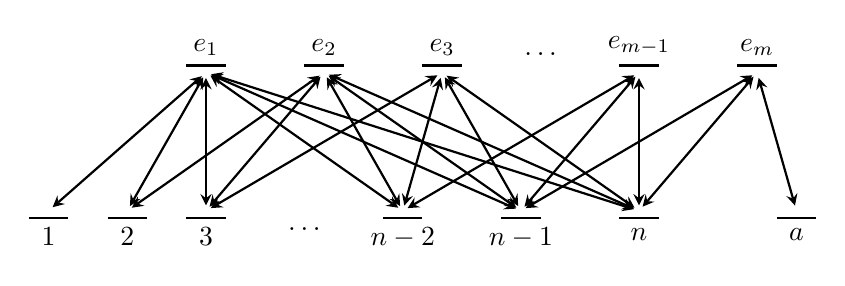
\begin{tikzpicture}[
      scale=0.5,
      level/.style={thick},
      virtual/.style={thick,densely dashed},
      trans/.style={thick,<->,shorten >=2pt,shorten <=2pt,>=stealth},
      classical/.style={thin,double,<->,shorten >=4pt,shorten <=4pt,>=stealth}]
   
    \draw[level] (4cm,-11em) -- (5cm,-11em) node[midway,below] {$\ket{1}$};
    \draw[level] (6cm,-11em) -- (7cm,-11em) node[midway,below] {$\ket{2}$};
    \draw[level] (8cm,-11em) -- (9cm,-11em) node[midway,below] {$\ket{3}$};
    \draw (11cm,-11em)  node[below] {$\dots$};
    
    \draw[level] (13cm,-11em) -- (14cm,-11em) node[midway,below] {$\ket{n-2}$};
    \draw[level] (16cm,-11em) -- (17cm,-11em) node[midway,below] {$\ket{n-1}$};
    \draw[level] (19cm,-11em) -- (20cm,-11em) node[midway,below] {$\ket{n}$};
    \draw[level] (23cm,-11em) -- (24cm,-11em) node[midway,below] {$\ket{a}$};
    
  % Draw the energy levels.
    \draw[level] (8cm,0em) -- (9cm,0em) node[midway,above] {$\ket{e_1}$};    
   	\draw[level] (11cm,0em) -- (12cm,0em) node[midway,above] {$\ket{e_2}$};
   	\draw[level] (14cm,0em) -- (15cm,0em) node[midway,above] {$\ket{e_3}$};
    \draw (17cm, 0em) node[above] {$\dots$};
    
    \draw[level] (19cm,0em) -- (20cm,0em) node[midway,above] {$\ket{e_{m-1}}$};
    \draw[level] (22cm,0em) -- (23cm,0em) node[midway,above] {$\ket{e_{m}}$};
    % Draw the transitions.
   % e_0
    \draw[trans] (8.5cm,-0.5em) -- (4.5cm,-10.5em) node[midway,left] {};
    \draw[trans] (8.5cm,-0.5em) -- (6.5cm,-10.5em) node[midway,left] {};
    \draw[trans] (8.5cm,-0.5em) -- (8.5cm,-10.5em) node[midway,left] {};
    \draw[trans] (8.5cm,-0.5em) -- (13.5cm,-10.5em) node[midway,left] {};
	\draw[trans] (8.5cm,-0.5em) -- (16.5cm,-10.5em) node[midway,left] {};
    \draw[trans] (8.5cm,-0.5em) -- (19.5cm,-10.5em) node[midway,left] {};
       
   % e_1
    \draw[trans] (11.5cm,-0.5em) -- (6.5cm,-10.5em) node[midway,left] {};
    \draw[trans] (11.5cm,-0.5em) -- (8.5cm,-10.5em) node[midway,left] {};
        \draw[trans] (11.5cm,-0.5em) -- (13.5cm,-10.5em) node[midway,left] {};
	\draw[trans] (11.5cm,-0.5em) -- (16.5cm,-10.5em) node[midway,left] {};
    \draw[trans] (11.5cm,-0.5em) -- (19.5cm,-10.5em) node[midway,left] {};
    
    % e_2
    \draw[trans] (14.5cm,-0.5em) -- (8.5cm,-10.5em) node[midway,left] {};
        \draw[trans] (14.5cm,-0.5em) -- (13.5cm,-10.5em) node[midway,left] {};
	\draw[trans] (14.5cm,-0.5em) -- (16.5cm,-10.5em) node[midway,left] {};
    \draw[trans] (14.5cm,-0.5em) -- (19.5cm,-10.5em) node[midway,left] {};


	% e_n-1
	        \draw[trans] (19.5cm,-0.5em) -- (13.5cm,-10.5em) node[midway,left] {};
			\draw[trans] (19.5cm,-0.5em) -- (16.5cm,-10.5em) node[midway,left] {};
   			 \draw[trans] (19.5cm,-0.5em) -- (19.5cm,-10.5em) node[midway,left] {};

	% e_n
				\draw[trans] (22.5cm,-0.5em) -- (16.5cm,-10.5em) node[midway,left] {};
   			 \draw[trans] (22.5cm,-0.5em) -- (19.5cm,-10.5em) node[midway,left] {};
   			 
   			 \draw[trans] (22.5cm,-0.5em) -- (23.5cm,-10.5em) node[midway,left] {};


    \end{tikzpicture}
    
    \caption{big mess}
\end{figure}

The system is given by $m$ ''excited'' states $\ket{e_i},\,i = 0,1,\dots,m$ and $n$ ''ground'' states labeled $\ket{i},\,i = 1,2,\dots,n$ and one auxiliary state $\ket{a}$. The number of states always follows that $n-m = 1$.(if auxiliary state is counted as a ''ground state'' it is = 2) So for $m = 5$ excited states there would be $n = 6$ ground states.
The transitions (except for auxialiary) occur only between excited states and ground states. the first excited state $e_1$ is connected to all ground states, $e_2$ is connected to all but $\ket{1}$, in general the excited state $\ket{e_i}$ is connected to the $(n - i)$th ground states with the highest label. Unless when $i = m$, the excited state $\ket{e_m}$ which is connected to the two highest labeled ground states and the auxiliary state $\ket{a}$.

This is the standard basis $\{e_1,e_2,\dots,e_m,1,2,\dots,n,a\}$, it is possible define a new basis, the dark state basis given by $\{e_1,e_2,\dots,e_m,b_1,b_2,\dots,b_{m},a,d\}$.

Given a dark state on the form 
\begin{equation}
\ket{d} = c_1\ket{1} + c_2\ket{2} + c_3\ket{3} \dots + c_{n}\ket{n},\, |c_1|^2 + |c_2|^2 + \dots + |c_{n}|^2 = 1
\end{equation}
from this dark state one could recursivly define $n-1 = m$ bright states.
Starting from
\begin{equation}
\ket{b_1} = N_1\left(-c_2\ket{1} + c_1\ket{2}\right)
\end{equation}
with $N_1$ being a normalization factor. Then choose additional bright states on the form
\begin{equation}
\begin{aligned}
&\ket{b_2} &=& N_2 \left(c_1\ket{1} + c_2\ket{2} + \Lambda_{1}^{(2)}\ket{2}  \right)
\\
&\ket{b_3} &=&  N_3 \left(c_1\ket{1} + c_2\ket{2} + \Lambda_{1}^{(3)}\ket{2} + \Lambda_{2}^{(3)}\ket{3} \right)
\\
&\;\;\vdots
\\
&\ket{b_{m-1}} &=& N_{m-1} \left( c_1\ket{1} + c_2\ket{2} + \Lambda_{1}^{(m-1)}\ket{2} + \Lambda_{2}^{(m-1)}\ket{3} + \dots + \Lambda_{m-2}^{(m-1)}\ket{m-1} \right)
\\
&\ket{b_{m}} &=& N_m \left( c_1\ket{1} + c_2\ket{2} + \Lambda_{1}^{(m)}\ket{2} + \Lambda_{2}^{(m)}\ket{3} + \dots + \Lambda_{m-2}^{(m)}\ket{m-1} + \Lambda_{m-1}^{(m)}\ket{m} \right).
\end{aligned}
\end{equation}
By this construction it is clear that $\ket{b_1}$ is orthogonal to all other bright states.

The coeffcients can be chosen in such a way that, in $\ket{b_2}$, the coeffcient $\Lambda_1^{(2)}$ can be chosen such that, $\bra{d}\ket{b_2} = 0$, and in $\ket{b_3}$, the coeffcient $\Lambda_1^{(3)}$ can be chosen such that, $\bra{b_2}\ket{b_3} = 0$ and $\Lambda_2^{(3)}$ such that $\bra{d}\ket{b_3} = 0$. By recursivly repeating this arugment one could see that it is possible to chose $m$ bright states, then by normalizing all the $N_i$ can be found, thus we have obtained $m$ orhonormal bright states, $\bra{b_i}\ket{b_j} = \delta_{ij}$.

The coeffcients $c_i$ can be parametrized by the euclidian components of the unit-$n$-sphere and a phase factor.

\begin{equation}
\begin{aligned}
c_1 &= \cos(\varphi_1)
\\ 
c_2 &= e^{i\theta_1}\sin(\varphi_1)\cos(\varphi_2)
\\ 
c_3 &= e^{i\theta_2}\sin(\varphi_1)\sin(\varphi_2)\cos(\varphi_3)
\\
&\hspace{2mm}\vdots
\\
c_{n-1} &= e^{i\theta_{n-1}}\sin(\varphi_1)\dots\sin(\varphi_{n-2})\cos(\varphi_{n-1})
\\
c_{n} &= e^{i\theta_{n}}\sin(\varphi_1)\dots\sin(\varphi_{n-2})\sin(\varphi_{n-1})
\end{aligned}
\end{equation}

$c_1$ does not need a phase factor since the overall phase of a state is non-measureable and can be chosen such that the first phase factor can be canceled. The remaining $\Lambda$ coefficients can be expressed in terms of the $c_i$.

In this newly defined space the Hamiltonian can be written as
\begin{equation}
H_d = \sum_{i = 1}^m \frac{\Omega_i(t)}{2}e^{-i\phi_i}\ket{b_i}\bra{e_i} + \frac{\Omega_a(t)}{2}\ket{a}\bra{e_n} +\;\text{h.c}
\end{equation}
with $\Omega_i$ being real-valued time dependent parameters and the $\phi_i$ time independent phase factors.



\begin{figure}[H]
    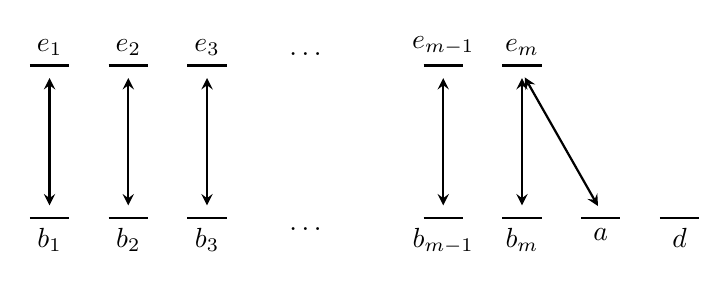
\begin{tikzpicture}[
      scale=0.5,
      level/.style={thick},
      virtual/.style={thick,densely dashed},
      trans/.style={thick,<->,shorten >=2pt,shorten <=2pt,>=stealth},
      classical/.style={thin,double,<->,shorten >=4pt,shorten <=4pt,>=stealth}]
    \draw[level] (0cm,-11em) -- (1cm,-11em) node[midway,below] {$\ket{b_1}$};
    \draw[level] (2cm,-11em) -- (3cm,-11em) node[midway,below] {$\ket{b_2}$};
    \draw[level] (4cm,-11em) -- (5cm,-11em) node[midway,below] {$\ket{b_3}$};
    \draw (7cm,-11em)  node[below] {$\dots$};    
    \draw[level] (10cm,-11em) -- (11cm,-11em) node[midway,below] {$\ket{b_{m-1}}$};
    \draw[level] (12cm,-11em) -- (13cm,-11em) node[midway,below] {$\ket{b_m}$};
    \draw[level] (14cm,-11em) -- (15cm,-11em) node[midway,below] {$\ket{a}$};
    \draw[level] (16cm,-11em) -- (17cm,-11em) node[midway,below] {$\ket{d}$};
    
  % Draw the energy levels.
    \draw[level] (0cm,0em) -- (1cm,0em) node[midway,above] {$\ket{e_1}$};    
   	\draw[level] (2cm,0em) -- (3cm,0em) node[midway,above] {$\ket{e_2}$};
   	\draw[level] (4cm,0em) -- (5cm,0em) node[midway,above] {$\ket{e_3}$};
    \draw (7cm, 0em) node[above] {$\dots$};
    \draw[level] (10cm,0em) -- (11cm,0em) node[midway,above] {$\ket{e_{m-1}}$};
    \draw[level] (12cm,0em) -- (13cm,0em) node[midway,above] {$\ket{e_{m}}$};
        
    % Draw the transitions.
   % e_1
    \draw[trans] (0.5cm,-0.5em) -- (0.5cm,-10.5em) node[midway,left] {};     
   % e_2
    \draw[trans] (2.5cm,-0.5em) -- (2.5cm,-10.5em) node[midway,left] {};
    % e_3
    \draw[trans] (4.5cm,-0.5em) -- (4.5cm,-10.5em) node[midway,left] {};
	% e_m-1
	\draw[trans] (10.5cm,-0.5em) -- (10.5cm,-10.5em) node[midway,left] {};
	% e_m
	\draw[trans] (12.5cm,-0.5em) -- (12.5cm,-10.5em) node[midway,left] {};
	\draw[trans] (12.5cm,-0.5em) -- (14.5cm,-10.5em) node[midway,left] {};
    \end{tikzpicture}  
    \caption{less mess}
\end{figure}


With this Hamiltonian $m$ dark paths can be constructed, and must fullfill $\bra{D_i(t)}H_d\ket{D_i(t)} = 0, i = 1,2,\dots,m$ and $\bra{D_i(t)}\ket{D_j(t)} = \delta_{ij}$.\\
The dark paths can be parametrized by two functions $u(t),v(t)$ that satisfy the conditions $u(0) = v(0) = u(T) = v(T) = 0$,  will have the form
\begin{equation}
\begin{aligned}
\ket{D_i(t)} &= \cos u e^{-i\phi_i}\ket{b_i} + i\sin u \ket{e_1},\, i = 1,2,\dots,m-1
\\
\ket{D_m(t)} &= \cos u \cos v e^{-i\phi_n}\ket{b_m} - i\sin u \ket{e_m} - \cos u \sin v \ket{a}
\end{aligned}
\end{equation}
The dark paths start in the bright state and travels along a curve where the expectation value of the energy is constantly $0$ and can thus be used non-adiabatically.

By using these states one can reverse engineer the Hamiltonian using the schrödinger equation to determine $\Omega_i$ and $\Omega_a$ since 
\begin{equation}
i\pdv{}{t}\ket{D_i(t)} = H_d\ket{D_i(t)},\; i = 1,2,\dots,m
\end{equation}
a calulation \note{actually do the calculation} yields
\begin{equation}
\begin{aligned}
\Omega_1(t) &= -2\dot{u}
\\ 
\Omega_2(t) &= -2\dot{u}
\\
&\hspace{2mm}\vdots
\\
\Omega_{m-1}(t) &= -2\dot{u}
\\
\Omega_m(t) &= 2\left(\dot{v}\cot u\sin v + \dot{u}\cos v \right)
\\
\Omega_a(t) &= 2\left(\dot{v}\cot u\sin v - \dot{u}\sin v \right)
\end{aligned}
\end{equation}

The time evolution is split into $k$ loops, each loop with two pulses, $0 \longrightarrow T/2$ and $T/2 \longrightarrow T$. The relevant part of the time evolution operator for one loop is  
$U_1(T/2,0) = \ket{d}\bra{d} -i\sum_{i = 1}^m \ket{e_i}\bra{b_i},\, \phi_i = 0, i = 1,2,\dots,n$ and $U_2(T,T/2) = \ket{d}\bra{d} + i\sum_{i = 1}^m e^{i\gamma_i}\ket{b_i}\bra{e_i},\, \phi_i = 0, i = 1,2,\dots,n $
The full operator for one loop is then given by 
\begin{equation}
U = U_2U_1 = \ket{d}\bra{d} + \sum_{i = 1}^{m}e^{i\gamma_i}\ket{b_i}\bra{b_i}.
\end{equation}
It is clear that $U$ is unitary in the subspace $\{d,b_1,b_2,\dots,b_n\}$

The unitary is parametrized by $3m = 3(n-1), n\geq 2$, parameters,
\begin{equation}
U(\varphi_1,\dots,\varphi_m,\theta_1,\dots,\theta_m,\gamma_1,\dots,\gamma_m) 
\end{equation} 

\note{The following part might not be 100\% correct, procced with caution!}

Now to perform a quantum gate one needs to apply $U$ $k$-times, $U_{tot} = U^k$, each time with a different set of parameters. This is due to the fact that just one loop does not have enough degrees of freedom to cover the dimensions of an $n-$dimensional qudit.

The dimensions of a $n-$dim qudit is given by $\dim(SU(n)) = n^2 -1$ and each loop only carries $3(n-1)$ degrees of freedom. So the loop needs to be repeated $k$ times such that $3(n-1)k \geq n^2 -1$.
Lets call the dimension $n$ when $\frac{n^2-1}{3(n-1)}$ is an integer, a ''perfect'' dimension, since no degrees of freedom goes ''to waste'' so to speak. In Table \ref{tab:dim} it seems such that $n$ is perfect when $n = 3p + 2$, for any integer $p$.
A quick calulation shows
\begin{equation}
\frac{n^2 -1}{3(n-1)} = \frac{(3p+2)^2-1}{3((3p+2)-1)} = \frac{3(3p^2 + 4p + 1)}{3(3p+1)} = \frac{(3p + 1)(p + 1)}{(3p +1)} = p + 1
\end{equation}
and since $p$ is an integer, $p + 1$ is also always an integer.\\
\note{OBS! The $T$ gate is only defined for prime number dimensions... \citep{qudit}}
\begin{table}[H]
\centering 
\begin{tabular}{|c|c|c|c|c|}
\hline
$n$ & $3(n-1)$ & $n^2 - 1$ & $k$ & is perfect?\\
\hline
2& 3& 3& 1& yes\\
3& 6& 8& 2& \\
4& 9& 15& 2& \\
5& 12& 24& 2& yes \\
6& 15& 35& 3& \\
7& 18& 48& 3& \\
8& 21& 63& 3& yes \\
9& 24& 80& 4& \\
10& 27& 99& 4& \\
11& 30& 120& 4& yes \\
12& 33& 143& 5& \\
\hline
\end{tabular}
\caption{Table for some dimensions.}
\label{tab:dim}
\end{table}

\begin{figure}[H]
\centering
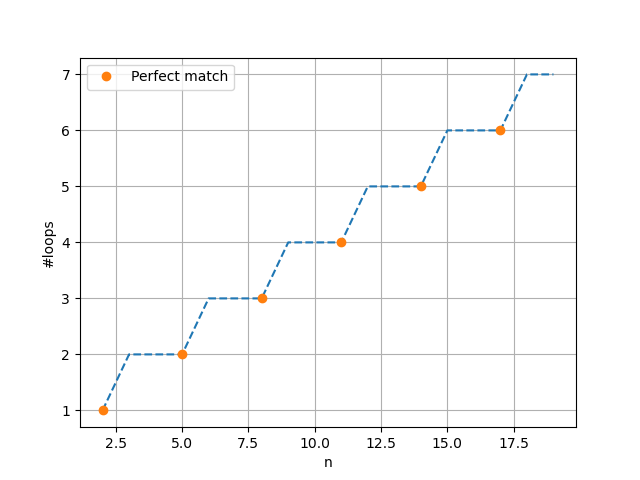
\includegraphics[scale=0.6]{figures/perfect_dim.png}
\end{figure}

This seems to hint that for when $n$ is perfect the amount of information has greater effciency since in higher dimensions more information can be contained but can be executed in the same number of loops as a non-perfect dim. 
\\ 
The quantum gate $U$ can be simulated simply as a function of a linear combination of the dark state and dark paths
\begin{equation}
\ket{\psi(t)} = f_0\ket{d} + \sum_{i = 1}^{m}f_i\ket{D_i(t)}, t \in [0,T]
\end{equation}
where the coeffcient can be solved for by choosing an initial state $\ket{\psi(0)}$. This corresponds to one loop, by using $\ket{\psi(T)}$ as an initial state for the next loop one can simulate $U^k$ by iterating this method.





